% !TEX encoding = UTF-8
% !TEX TS-program = pdflatex
% !TEX root = ../tesi.tex

%**************************************************************
\chapter{Design and development}
\label{cap:design-development}
%**************************************************************

\intro{In this chapter I will explain my technology choices and how these influenced the development of the final application.}\\

%**************************************************************
\section{Technology and tools}
\label{sec:technology-tools}

In the following I will introduce the technologies I used and the reasons behind their choice.

\subsection*{Deep learning framework}
There are many popular deep learning frameworks out there, but I was asked to choose between \emph{MXNet} and \emph{TensorFlow} after experimenting with both for bit. Keep in mind that I was required to use \emph{YOLO v3} as my \emph{convolutional neural network} and it influenced greatly my final choice. Furthermore, due to Python being predominant in deep learning, I had little freedom in choosing a programming language\footnote{Actually I did try Scala APIs on MXNet, but I had little success with them due to the restricted set of functionality provided when compared to Python.}

\subsubsection*{MXNet and Gluon CV}
\emph{MXNet} is an open source deep learning framework developed by Apache. It supports various languages, but the most extensive toolkit is written in Python; in particular MXNet Python provides \emph{Gluon}, a high-level API that allows to easily build and train \emph{deep neural networks}. \emph{Gluon} is also used by \emph{Gluon CV}, a \emph{computer vision} toolkit that provides out-of-the-box implementation of several \emph{neural networks}, pre-trained models and even complete \emph{training scripts}. In particular \emph{YOLO v3} is well supported and many useful tutorials are available. \\
Both \emph{MXNet} and \emph{Gluon CV} can be installed from \emph{\gls{PyPI}}\textsubscript{g} with \emph{\gls{Pip}}\textsubscript{g}. \\
There are minor compatibility issues since \emph{Gluon CV} 0.3.0 requires \emph{MXNet} 1.3.0 and later.

\subsubsection*{TensorFlow}
\emph{TensorFlow} is an open source machine learning framework developed by Google Brain. It supports various language, but as common in this field the most extensive one is written in Python. \emph{TensorFlow} is compatible with \emph{Keras}, a high-level API to build and train \emph{deep neural networks}; sadly \emph{Keras} does not provide any network model for \emph{computer vision}. \\
When looking to \emph{YOLO v3} support I explored \emph{TensorFlow}'s \emph{GitHub} repository, where they host some research projects developed and maintained by independent researchers and not officially supported or distributed in release branches. Among the \emph{computer vision} models on there I did not find \emph{YOLO v3}, but I took my time to experiment with a \emph{SSD} model just to see if \emph{TensorFlow} was worth anyway. \\
\emph{TensorFlow} can be installed from \emph{PyPI} with \emph{Pip}, but the research toolkit cannot.

\subsubsection*{My choice}
Since \emph{MXNet}'s \emph{Gluon CV} provides a comprehensive toolkit with models, scripts and utilities to train and infer \emph{YOLO v3} \emph{convolutional neural networks}, it easily became my framework of choice. \\
As I said I tried \emph{TensorFlow} with \emph{SSD}, but it was a low-level implementation that relied a lot on a \emph{\gls{Jupyter notebook}}\textsubscript{g} and it was not suitable for the goals of my project.

\subsection*{IntelliJ IDEA}
I used \emph{\gls{IntelliJ IDEA}}\textsubscript{g} IDE to write my code and I installed \emph{PEP} \emph{Python} linter plugin to check my code style. \\


\subsection*{GitLab}
I was given access to a \emph{\gls{GitLab}}\textsubscript{g} repository to version control my work and I used \emph{IntelliJ IDEA}'s built-in \emph{Git} interface to access it.


\subsection*{Docker}
\emph{\gls{Docker}}\textsubscript{g} is a software application to create containers, virtual environments with their own operative system and tools installed. Containers can communicate with each other and to the outer world through ports, and can mount hard drives when consistent memory is needed. \\
I used it in various steps of my project's development; at first I created a \emph{Linux} \emph{Docker} container to set up a \emph{Python 2.7} and \emph{MXNet} environment to run my code. I also created a \emph{MongoDB} instance on another container. \\
At some point I even dockerized my application to run it on \emph{AWS}.


\subsection*{OpenAPI + Swagger}
Thron works with a service architecture, so I was asked to follow it when developing my inference web application. I wrote a \emph{\gls{YAML}}\textsubscript{g} \emph{\gls{OpenAPI}s}\textsubscript{g} using \emph{\gls{Swagger}}\textsubscript{g} to declare my application's interface, which also served as documentation.

\subsection*{Flask + Connexion}
My server application for inference is written in \emph{Python}, so I set up a \emph{\gls{Flask}}\textsubscript{g} server to host it. The \emph{Flask} needed to adhere to the operations and responses I declared on the \emph{OpenAPI}; matching everything manually would be a tedious job, but thankfully \emph{Zalando}\footnote{E-commerce platform.} developed a framework called \emph{Connexion}\footnote{Zalando Connexion repository: \url{https://github.com/zalando/connexion}} that, provided the \emph{OpenAPI} automatically handles the HTTPs requests and maps them to your Python functions.

\subsection*{Postman}
I used \emph{\gls{Postman}}\textsubscript{g} to send \emph{HTTP} request to my web server and check its behavior.

\subsection*{MongoDB + Robo 3T}
I set up a \emph{\gls{MongoDB}}\textsubscript{g} instance in a \emph{Docker} container to model a queue I needed in my inference application, and I used the \emph{Pymongo}\footnote{Pymongo website: \url{https://api.mongodb.com/python/current/}} toolkit to work with it from my server application. \\
To easily access and manage my database, I used \emph{\gls{Robo 3T}}\textsubscript{g} client.

\subsection*{AWS SageMaker}
I experimented with \emph{AWS} \emph{\gls{SageMaker}}\textsubscript{g} to test whether a \emph{YOLO v3} training script could easily take advantage of \emph{AWS}'s computational power in a future production environment.




%**************************************************************


%**************************************************************
\section{Design}
\label{sec:design}
In this section I will cover the design choices I made while developing my application.

\subsection{Overview}
As stated before, THRON'S \emph{DAM} categorizes images inserted by the clients to make their access easier. Details about how these images are stored in a non-relational database are irrelevant for my project, and I actually do not know them. However, how a database export is structured and what it contains do is important and had major influence in some implementation choices. \\
A database export is a  \emph{\gls{Json lines file}}\textsubscript{g} where each line represent a valid Json file containing information about an image in the database; the covered fields are the following:
\begin{itemize}
	\item ID: image unique identifier;
	\item Client ID: client identifier\footnote{Thron has several clients and often uses client ID based sharding techniques to run services in order to guarantee various levels of fairness.}; the goal is to construct a custom dataset for detection for each client's needs so this parameter is vital;
	\item Url: location where the image is stored, likely an \emph{Amazon S3}\footnote{AWS cloud storage service; Amazon S3 website: \url{https://aws.amazon.com/s3}} cloud storage location.
	\item Data: image properties relevant in the dataset context such as \emph{bounding boxes} coordinates and classes.
\end{itemize}


\subsection{Dataset creation}

\subsubsection{Format choice}
To train the network model for my prototype I was given a dataset created by one of my co-workers; his format of choice\footnote{Each raw image in the dataset was labeled by an XML file containing the image size, bounding boxed and classes.}, however, it was not compatible with my framework so I had to convert it with a script. \\
\emph{Gluon CV} provides modules to load a custom dataset from two different formats:
\begin{itemize}
	\item Record file format; this format is composed by two different files, a \emph{*.rec} binary file, containing the encoded images and their labels, and a \emph{*.idx} file containing the indexes to provide random access to the binary;
	\item Pure text file format; this format is composed by a \emph{*.lst} file\footnote{It is a text file readable as a tab-separated \emph{*.csv file.}}. Each line of this file contains the path to an image on disk and the labels describing its bounding boxes.
\end{itemize}


\begin{figure}[htbp]
\begin{center}
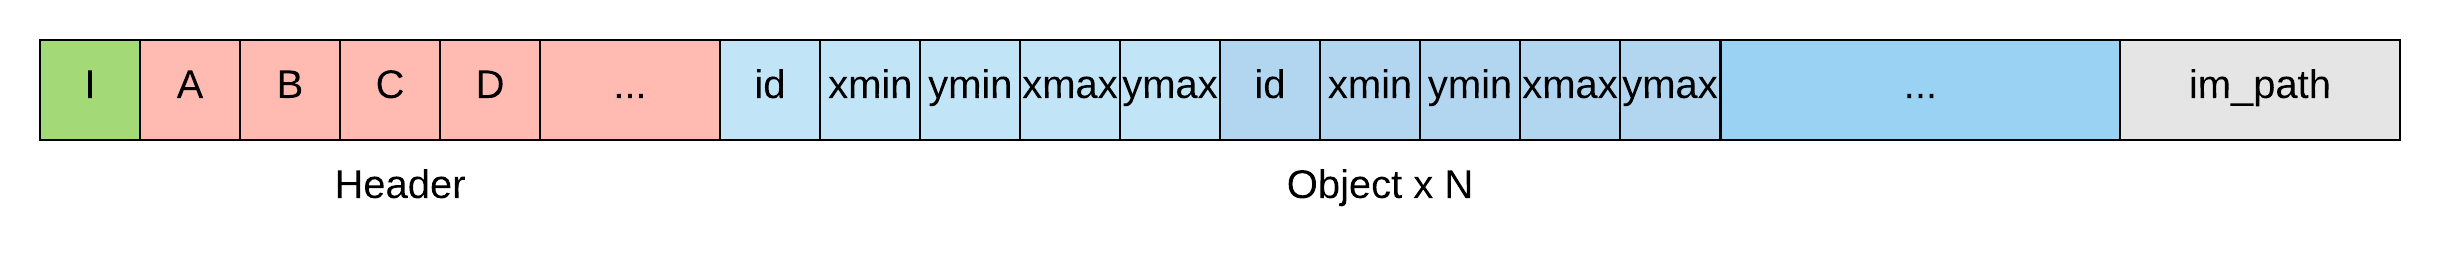
\includegraphics[width=\textwidth]{immagini/pictures/detection_label.png}
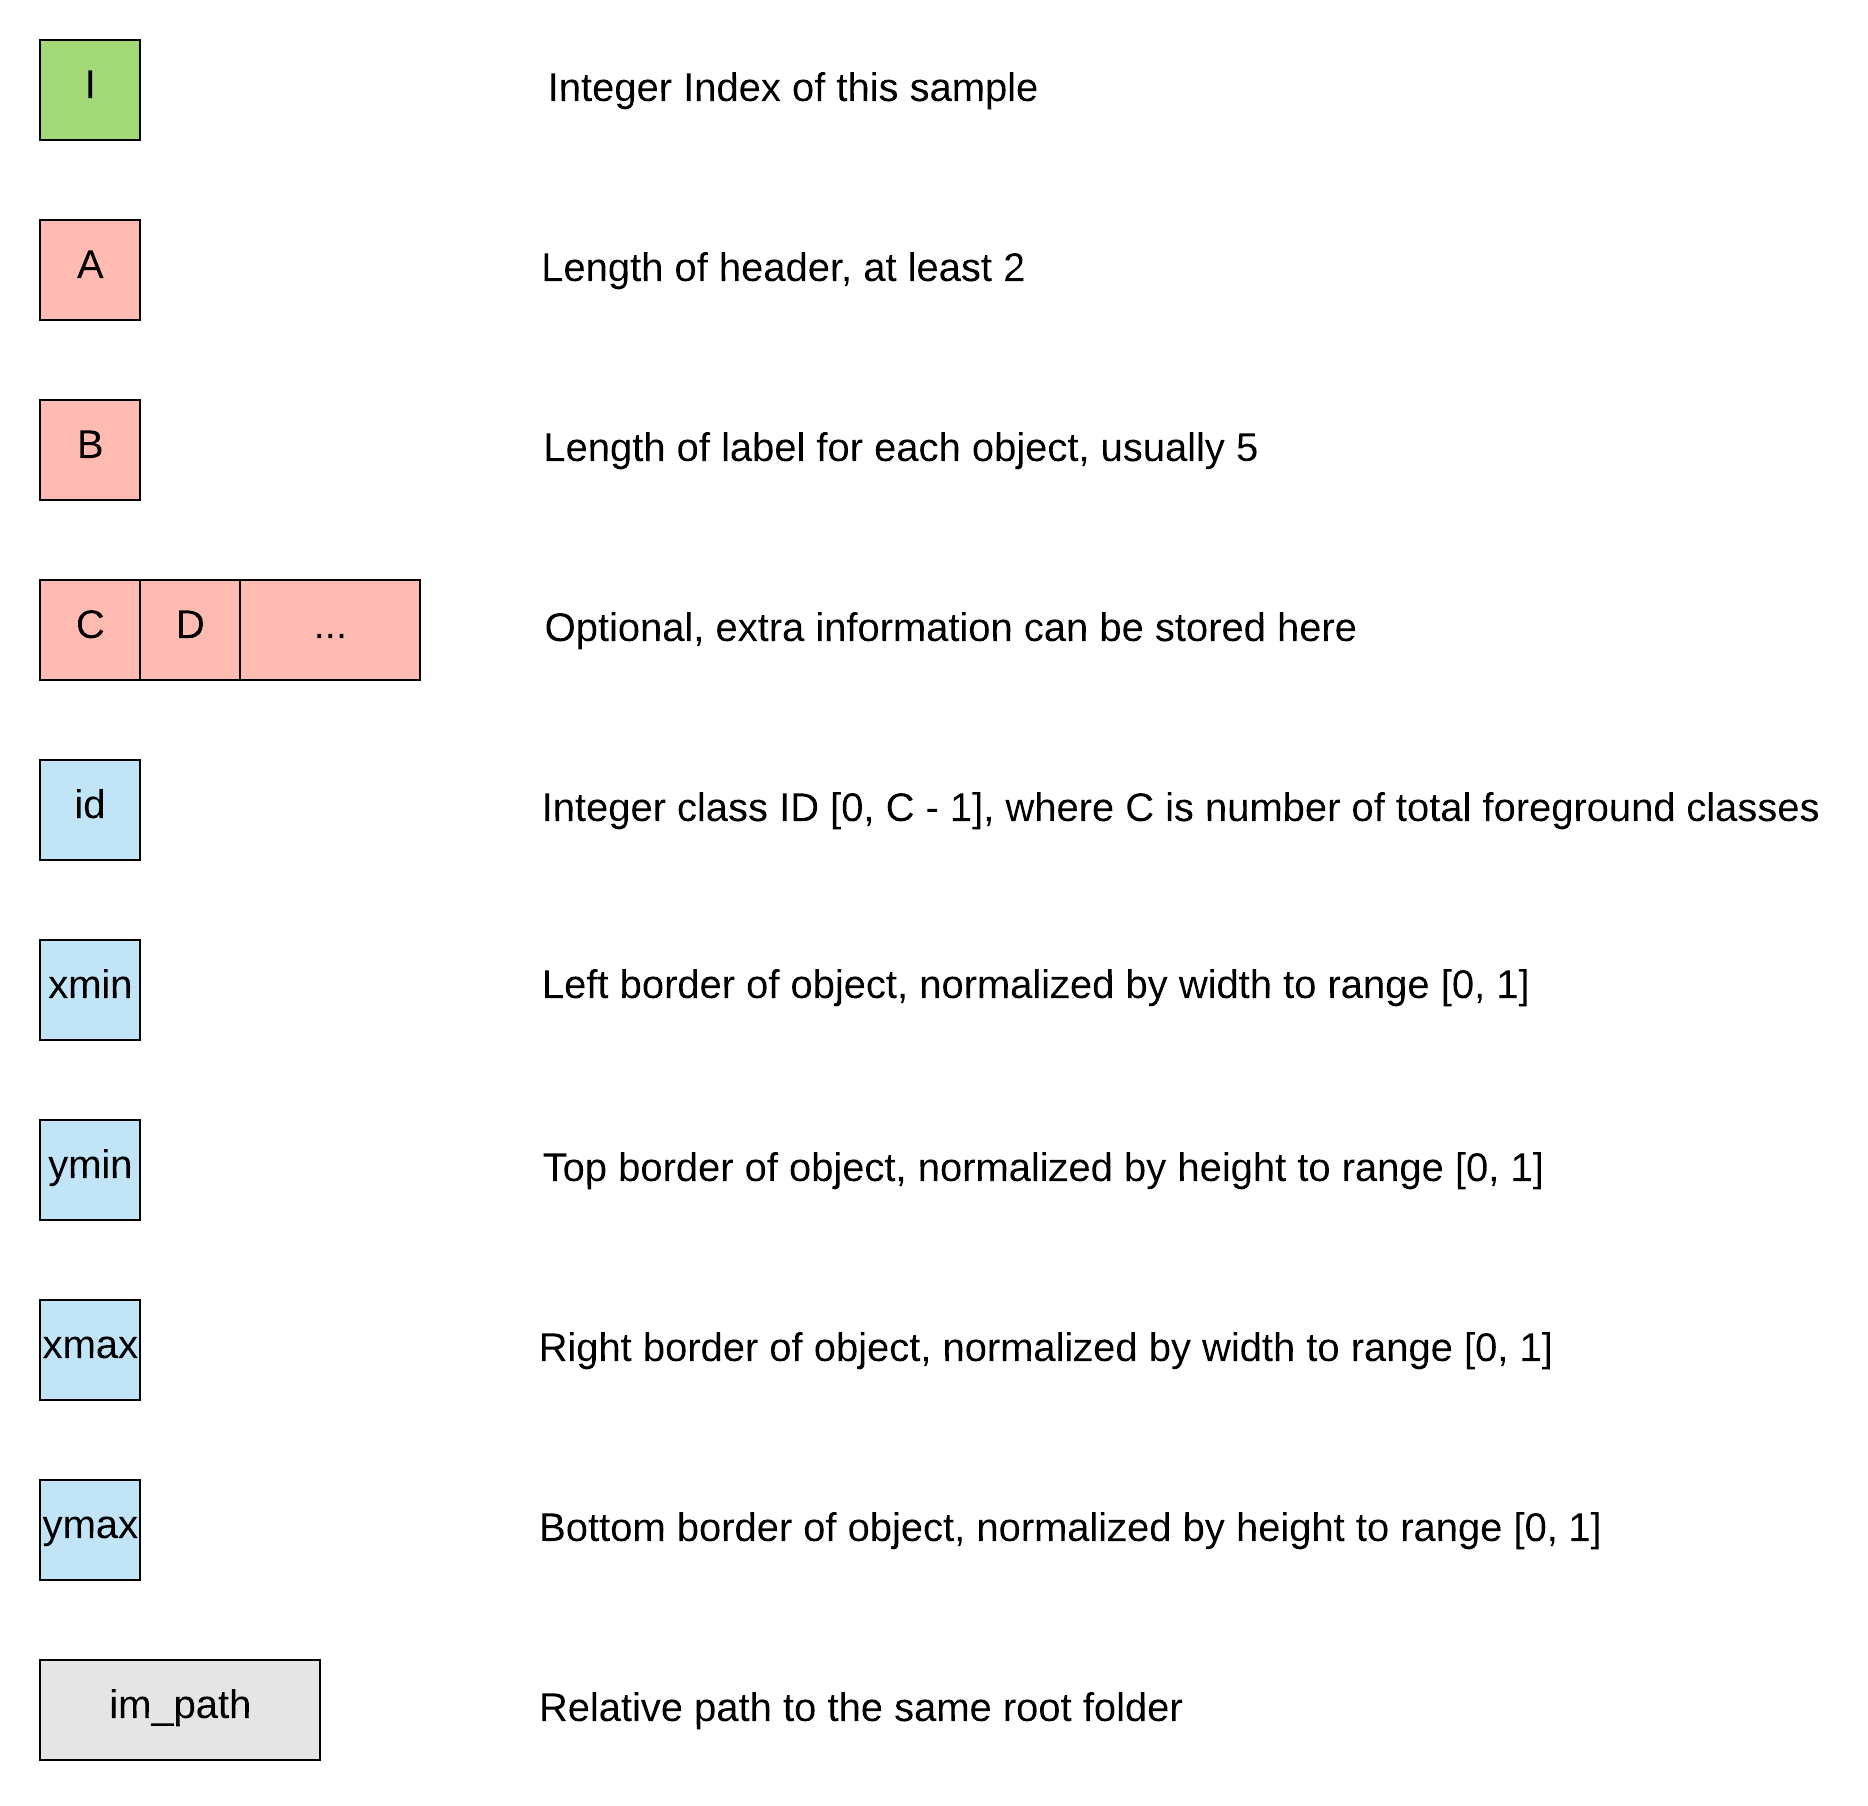
\includegraphics[width=\textwidth]{immagini/pictures/detection_label_detail.png} 
\caption{Structure of a \emph{*.lst} file containing dataset information.}
\end{center}
\end{figure}

The record file format allows faster training, but I chose to use the \emph{*.lst} file format instead because it allows you to work directly from raw images without prior computation. There are two main reason behind my choice:
\begin{enumerate}
	\item The production training process should run on \emph{AWS SageMaker}, which reads input data from an \emph{Amazon S3}; Thron already uses \emph{S3} so uploading the training on a dedicated bucket on there would be the easiest approach;
	\item In production environment the datasets should be created from \emph{Json lines file} database exports, so simply converting the \emph{Json lines} content describing the bounding boxes for each image to an \emph{*.lst} would be the easiest and fastest approach.
\end{enumerate}



\subsubsection{Dataset creation approach}
The dataset-creation module I designed takes a \emph{Json lines} database export file as its input and creates a \emph{*.lst} for each \emph{client ID} found in the \emph{Json lines}. The module also provides a function to split the dataset into \emph{training dataset} and \emph{validation dataset} after creation and saves an additional text file containing statistics about the dataset\footnote{These statistics include number of images, number of classes, cardinality and density.}. I chose to keep the creation of the full dataset and splitting it separated, as it is common practice to split the dataset right before training. \\
To track the class names with their numerical encoding used in the \emph{*.lst} dataset a \emph{*.txt} calles \emph{synset.txt} is used. This file must be created manually.


\subsection{Training}
Model training for my \emph{YOLO v3} network can be executed as a stand-alone \emph{Python} script. This file receives as an input the \emph{training} and \emph{validation} datasets in \emph{*.lst} format and the \emph{synset.txt} file. \\
My script actually performs \emph{transfer learning} instead of training from scratch due to the better performances achievable this way; the base network is a YOLO v3 Darknet53\footnote{YOLO v3 convolutional neural network built on top of a Darket classifier composed by 53 layers} pre-trained on the \emph{VOC} dataset; the \emph{VOC} weights are provided by the \emph{Gluon CV} toolkit and should cover classes general enough to prove useful in most cases.

\subsubsection{Hyperparameters}
My scripts accepts arguments to tune the training \emph{hyperparameters}. Follows the hyperparameters list and their description:
\begin{itemize}
	\item Data shape: input data shape; the shortest side of each image will be resized to match this value. Accepted values are 320, 416 and 608 (32 multiples) and it defaults to 416;
	\item Batch size: number of images in each computing batch. It must be tuned accordingly to your hardware as a batch size to big would trigger a bus error. It defaults to 8 (which works for CPU), but with GPU training you might be able to use a bigger size such as 32;
	\item Workers: number of workers used for training. You must tune it accordingly to your hardware as a number too high might result in a thread error;
	\item Gpus: numbers of the GPUs to use as a comma separated list of integers; to train on CPU leave this argument empty;
	\item Epochs: number of epochs to perform;
	\item Learning rate: speed at which your model learns the dataset content. A high learning rate makes you model learn quicker, but might result in overfitting;
	\item Learning rate decay rate: speed at which your learning rate decays;
	\item Learning rate decay epoch: epoch interval where your learning rate should decrease;
	\item Momentum: stochastic gradient descent momentum;
	\item Syncbn: argument to synchronize devices when training in parallel.
\end{itemize}


\subsubsection{Model export}
There are two ways to export a trained (or partially trained) network:
\begin{itemize}
	\item Saving weights: it is possible to set the network weights as a \emph{*.PARAMS} binary file every set epoch; this type of file is mostly used as a training checkpoint to resume training from later.
	\item Network export: it is possible to set an export epoch where both the network architecture with adjusted top layers and its weights are exported. The network itself is saved as a \emph{*.json} file describing its layers while the weights are saved as a \emph{*.PARAMS} similar to the checkpoint file. These files are coupled and must be used together to load the trained network; this export approach is used when you want to save a model to use for inference, as it can be loaded from different languages other that \emph{Python}.
\end{itemize}

\subsubsection{Resume training}
Since training demands a lot of computational power, it is useful to be able to stop a training process in order to resume it later. The following arguments allows you to load weights from a training checkpoint to resume training:
\begin{itemize}
	\item Resume: path to the \emph{*.PARAMS} binary file containing the training checkpoint;
	\item Start epoch: epoch where training should be resumed.
\end{itemize}
It is important to load a checkpoint \emph{*.PARAMS} binary file to resume training as the model export \emph{*.PARAMS} binary file cannot be loaded without its paired \emph{*.json}.

\subsection{Inference service}
While training usually requires GPU power to speed up the process, inference can be reasonably done on CPU, so I decided to keep my training script and my inference script separated.

\subsubsection{RESTful Architecture}
My inference request server uses a\emph{\gls{RESTful API}}\textsubscript{g} architecture that I designed using the API first approach; specifically, I wrote my \emph{OpenAPIs} using the \emph{Swagger}. To implement my APIs I took advantage of \emph{Zalando}'s \emph{Connexion}, a framework based on \emph{Flask} that tracks the operations declared in the OpenAPI to the application, validates the HTTP request exchange by comparing the actual Json content to what is declared in the API and manages error messages\footnote{Since I used \emph{Connexion} instead of a pure \emph{Flask} server application I couldn't override the standard HTTP error messages}. \\
To increase decoupling I kept my server interface separated from its implementation; in fact operations are declared in a \emph{JobOpsMongo} module called by the server interface via a \emph{JobService} module. I followed this decoupling approach for both \emph{MongoDB} related operations and \emph{MXNet} inference related operations, but the latter aren't directly called by the inference request server but are used by a queue consumer I did not implement and that potentially resides on AWS.

\begin{figure}[htbp]
\begin{center}
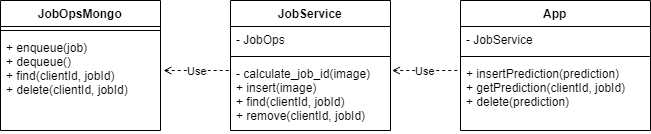
\includegraphics[width=\textwidth]{immagini/pictures/jobops.png} 
\caption{UML describing the relationship between the server application (App class) and the implementation of its methods.}
\end{center}
\end{figure}

Basically the server's job is to accept and manage inference requests by inserting them into a \emph{MongoDB} queue; from there a consumer will dequeue them and run the actutal inference. \\
HTTP requests work with \emph{Json} objects which, despite \emph{Connexion}'s automatic conversion into \emph{Python} dictionaries, still require tedious syntax to access their fields. On the other hand \emph{MongoDM} indexes its content in \emph{Json} format.
Since working with different formats of data would unnecessarily increase the application's complexity, I found it useful to model \emph{Python} class objects to reflect what was declared in the \emph{OpenAPI} and use them to work within the logic modules. My approach while designing these classes was to roughly follow the structure I declared in the OpenAPI, adding further information that could be useful inside the application, and to provide object creation, serialization\footnote{From \emph{Python} object to \emph{Json}} and deserialization \footnote{From \emph{Json} to \emph{Python} objects.} methods to quickly convert between  \emph{Python} objects, \emph{Python} dictionaries and \emph{Json}s as needed. \\

\subsubsection{Asynchronous computation}
While inference isn't to heavy on the computational side of the task, performing a prediction requires the trained network model to be loaded into memory and, since each model occupies over 250MBs of space, it is obvious that constantly switching from model to model would make the performance fall. The easiest solution to this problem is to perform inference by sharding the requests by client ID, so each batch of images runs on the same network model. A further advantage of client ID sharding is that it allows guarantee different levels of fairness accordingly to each client's service contract. \\
Since computation is obviously performed asynchronously, a client needs a way to retrieve its inference once it's completed. There are two main options to manage this: \emph{\gls{callback}s}\textsubscript{g} and \emph{\gls{polling}}\textsubscript{g}. I chose the latter because it comes more natural when working in a \emph{RESTful} environment, as after having inserted the new job in the queue the server can simply send a HTTP 202 Accepted response containing the address to check for the requested resource.

\subsubsection{Queue}
I modeled the queue on \emph{MongoDB}, as it provides an easy way to sort the elements in its collections by insertion time. Furthermore, contents in \emph{MongoDB} are represented as \emph{Json} objects, so it proved to be convenient to work with the objects I declared in the \emph{OpenAPI}. \\
The jobs queue is accessed by both my inference request server and a consumer, but I did not implement the latter.

\subsubsection{Inference work flow}
When a client needs an image to be inferred, it sends the server a HTTP Post request containing a \emph{Json} stating the URL to the image and a client ID; upon receiving the request the server creates a new inference request job and inserts it in a \emph{MongoDB} queue. If the insertion was successful, the server sends the client a HTTP 202 Accepted response, containing the URL where to check for the requested prediction; since computation runs asynchronously, the client might have to check several times for its requested inference result before it's actually available. \\
When the prediction is ready, the client can retrieve it from the given URL; inference contains the detected object classes, their confidence score\footnote{How much the network is confident the detected object belongs to the stated class; a higher score means higher confidence.} and their \emph{bounding boxes}, expressed in percentage on the image's size. \\
Predictions are executed by I consumer I did not implement.

\begin{figure}[htbp]
\begin{center}
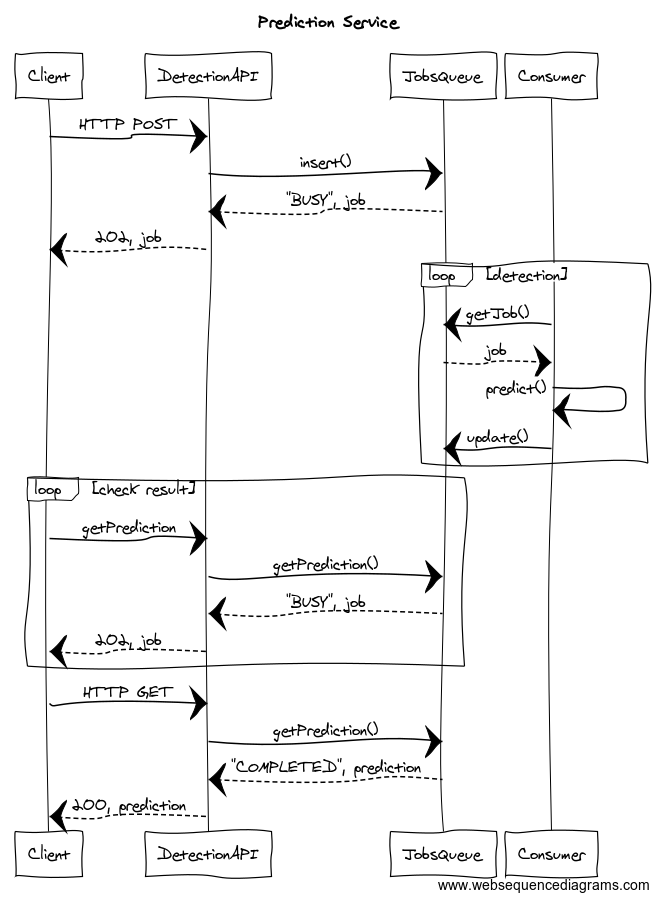
\includegraphics[width=\textwidth]{immagini/pictures/flow.png} 
\caption{UML flow chart displaying the HTTP message exchange in the application.}
\end{center}
\end{figure}


\subsubsection{Unit test}
I wrote unit tests that cover both the methods provided by the \emph{JobOpsMongo} module and the \emph{PredictionOpsMxnet} modules. 
While the \emph{JobOpsMongo} module was actually used by the application and I tried its functionality by sending HTTP requests via \emph{Postman} as well, the \emph{PredictionOpsMxnet} module has only been used by its unit tests. In fact, the \emph{PredictionOpsMxnet} module provides the inference methods that the consumer should use, but I did not implement it because it should potentially run on \emph{AWS} and therefore requires specific coding.

\subsection{Standalone inference script}
Before designing and developing the inference request server application, I wrote a \emph{Python} standalone script to perform inference on an image. This script takes the image path and the network model to use as arguments, and then run inference. The result is composed by the classes of the detected objects, their \emph{bounding boxes} and their confidence score; furthermore the inference script saves a copy of the input image where it draws\emph{To edit images I used Python PILLOW library. PILLOW website: \url{https://pillow.readthedocs.io/en/5.3.x/}} the \emph{bounding boxes} with their class and confidence score. \\
I used this inference script mainly when testing whether the network training was successful; since I used unlabeled data\footnote{Using dataset images for testing could give false performance, especially if overfitting has occurred.} for testing, visually checking whether the detection was accurate proved to be faster that automatizing the process, as classes and their \emph{bounding boxes} must be manually determined by a human anyway.
%**************************************************************

